\documentclass{standalone}
\usepackage{pgfplots}
\pgfplotsset{compat=newest}

\begin{document}
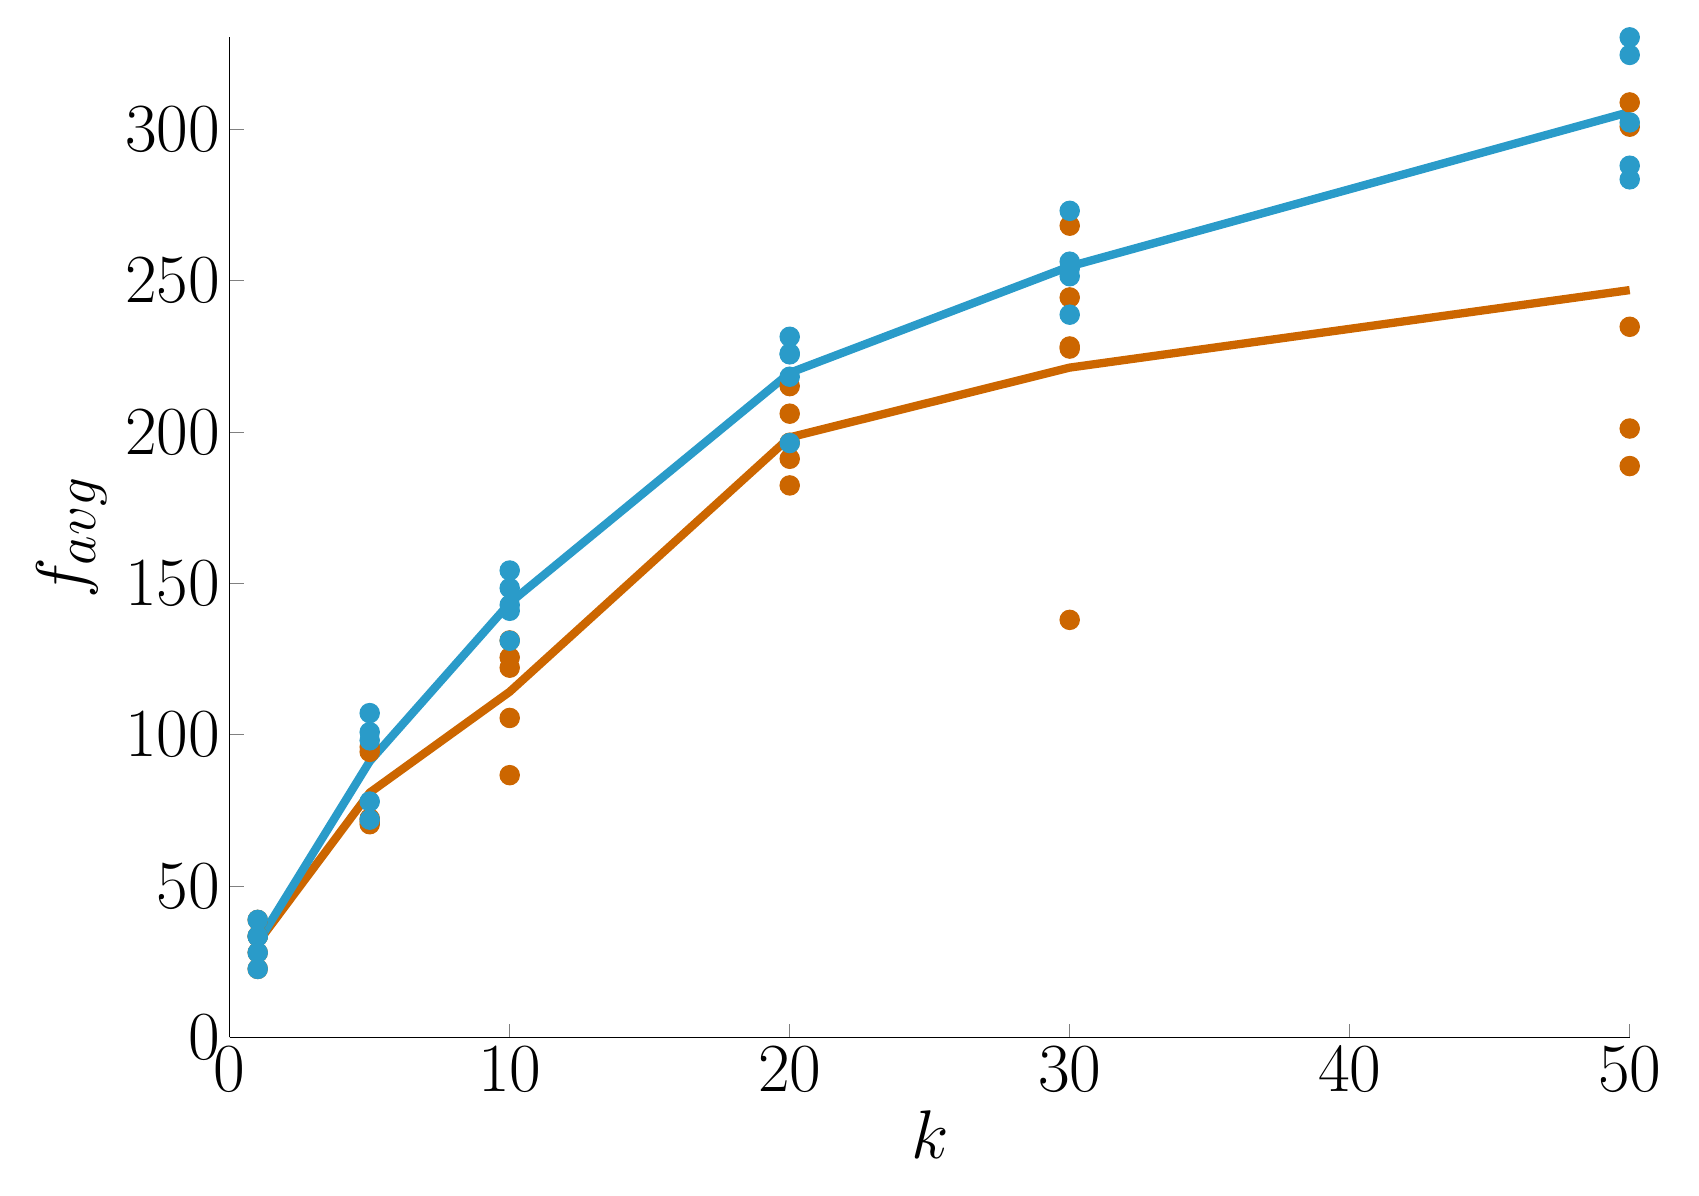
\begin{tikzpicture}

\begin{axis}[%
tick label style={font=\Huge},
label style={font=\Huge},
legend style={font=\Huge},
view={0}{90},
max space between ticks=50pt,
width=7in,
height=5in,
scale only axis,
xmin=0, xmax=50,
xtick={0, 10, 20, 30, 40, 50},
xlabel={$k$},
ymin=0, ymax=330.3,
%ytick={0, 200, 400, 600, 800, 1000},
ylabel={$f_{avg}$},
major tick length=5pt,
axis lines*=left,
legend cell align=left,
clip=false]

\addplot [
only marks,
mark=*,
mark size=3.5pt,
color=orange!80!black,
%solid,
%line width=2pt,
]
coordinates{
(1,22.6)(1,28.0)(1,33.4)(1,33.4)(1,38.8)(5,70.4)(5,71.2)(5,72.3)(5,94.3)(5,95.9)(10,86.6)(10,105.5)(10,122.1)(10,125.5)(10,131.1)(20,182.3)(20,191.1)(20,196.4)(20,206.0)(20,215.1)(30,137.9)(30,227.5)(30,228.2)(30,244.4)(30,268.1)(50,188.7)(50,201.1)(50,234.7)(50,300.8)(50,308.8)
};

\addplot [
only marks,
mark=*,
mark size=3.5pt,
color=cyan!80!black,
%solid,
%line width=2pt,
]
coordinates{
(1,22.6)(1,28.0)(1,33.4)(1,33.4)(1,38.8)(5,71.9)(5,77.9)(5,98.1)(5,100.8)(5,107.1)(10,131.0)(10,140.9)(10,142.8)(10,148.4)(10,154.2)(20,196.3)(20,218.2)(20,225.6)(20,225.9)(20,231.4)(30,238.7)(30,251.4)(30,253.9)(30,256.2)(30,273.0)(50,283.4)(50,287.9)(50,302.2)(50,324.5)(50,330.3)
};

\addplot [
color=orange!80!black,
solid,
line width=3pt
]
coordinates{
(1,31.24)(5,80.82)(10,114.16)(20,198.18)(30,221.22)(50,246.82)
};

\addplot [
color=cyan!80!black,
solid,
line width=3pt
]
coordinates{
(1,31.24)(5,91.16)(10,143.46)(20,219.48)(30,254.64)(50,305.66)
};


\end{axis}
\end{tikzpicture}
\end{document}
